% !TeX spellcheck = cs_CZ
%---------------------------------------------------------------------------------------------------
% file opamp.tex
%---------------------------------------------------------------------------------------------------
%================================ Kapitola: Zesilovače==============================================
\setchaptertoc
\chapter{Operační obvod}\label{aesIchIV}    
  \section{Ideální operační obvod}\label{aesIchIVsecI}
    \subsection{Paralelní operační obvod}
      \fbox{Napěťový invertor} ukazuje, že vstupní signálový proud může být generován také 
      synteticky, kombinací napěťového signálového zdroje a sériového rezistoru. Takovým způsobem 
      vytvořený \emph{napěťový invertor} na obr. * je jedním z nejčastějších operačních obvodů. 
      
      Vstupní napětí $u_s$ je celé vloženo na rezistor $R_1$ (jeho pravý konec je virtuálně 
      uzemněn) a vyvolává ekvivalentní vstupní proud $\frac{u_s}{R_1}$. Tento přitékající proud je 
      kompenzován proudem $-\frac{u_0}{R_2}$ odsávaným přes zpětnovazební rezistor $R_2$ do výstupu 
      operačního zesilovače $$\frac{u_s}{R_1}=-\frac{u_0}{R_2}.$$ Ideální operační rovnice
      \begin{equation}\label{AES:eq_opamp_inv02}
        u_0 = - \frac{R_2}{R_1}u_s.
      \end{equation}
      Vyjadřuje úměrnost signálových napětí $-u_0$ a $u_s$ velikostem přilehlých rezistorů $R_2$ a 
      $R_1$. Pro snadnější zapamatování se nabízí představa dvouramenné páky s délkami ramen $R_1$ 
      a $R_2$, otočné v bodě odpovídajícímu virtuální zemi, která přenáší výchylku $u_s$ levého 
      konce na výchylku $u_0$ pravého konce v opačné polaritě.

      \begin{figure}[ht!]
        \centering
        \subcaptionbox{$u_0 = -\dfrac{R_2}{R_1}u_s, \qquad R_{\parallel} = R_1, 
                  \qquad R_{\mathsf{O}\lvert} = s0$       \label{aes:fig075a}}
          {\luafigure[0.49]{opamp_inv01a.pdf}}                                    \\
        \subcaptionbox{ $u_0 = -\dfrac{R_2}{R_2+R_s}u_s$  \label{aes:fig075b}}
          {\luafigure[0.50]{opamp_inv01b.pdf}}             
        \caption{Napěťový invertor. Jeho mechanickou analogií je dvouramenná páka (a). Přítomnost 
                 vnitřního odporu signálového zdroje $R_s$ v operační rovnici je důsledkem 
                 konečného vstupního odporu $R_{\parallel} = R_1$ (b). }
        \label{aes:fig075}
      \end{figure}
      Zesílení napěťového invertoru 
      \begin{equation}\label{AES:eq_opamp_inv01}
        G_i = -\frac{R_2}{R_1},
      \end{equation} 
      je záporné a nastavitelné v širokých mezích od $0$ do $\infty$ výběrem rezistorů $R_1$ a 
      $R_2$. Zvláštním případem je jednotkový invertor se stejnými rezistory $R_1 = R_2$, který 
      prostě invertuje polaritu vstupního napětí: $$u_0 = - u_s, \qquad G_i = -1.$$
      
      Výstupní odpor napěťového invertoru je ideálně nulový. Jeho vstupní odpor však ztrácí onen 
      vyhranění charakter typický pro kanonické operační obvody a nabývá indiferentní velikosti 
      \begin{equation}\label{AES:eq_opamp_inv03}
        R_{\parallel} = R_1,
      \end{equation} 
      rovné velikosti virtuálně uzemněného rezistoru $R_1$.
      
      Napěťový invertor zatěžuje signálový zdroj (obr. *). To se projevuje poklesem svorkového 
      napětí signálového zdroje o úbytek na vnitřním odporu $R_s$, nebo jinak řečeno, přítomností 
      nedefinovaného a nestálého vnitřního odporu $R_s$ v operační rovnici invertoru:  
      \begin{equation}\label{AES:eq_opamp_inv04}
       u_0 = -\frac{R_2}{R_1 + R_s}u_s.
      \end{equation}      
      Taková vlastnost se obvykle považuje za nedostatek. 
            
    \subsection{Sériový operační obvod}
    
    \subsection{Složený operační obvod}
      Operační obvody, které není možné zahrnout do předcházejích dvou velkých tříd, se vyznačují:
        \begin{itemize}[noitemsep]
          \item signálovým buzením obou vstupů operačního zesilovače,
          \item násobnou zpětnou vazbou,
          \item kombinací záporné a kladné zpětné vazby,
          \item použitím několika operačních zesilovačů,
          \item nestandardním zapojením operačního zesilovače.
        \end{itemize}
      \subsubsection{Signálové buzení obou vstupů}
        \fbox{Rozdílový zesilovač} na obr. \ref{AES:fig_diff_opamp01} je lineární operační obvod se
        dvěma vstupy. Jeho výstupní napětí se najde superpozicí \cite[s.~126]{Dostal}. 
        
        Nechť působí napětí $u_1$ a napětí $u_2$ je nulové. Neinvertující vstup operačního 
        zesilovače je uzemněn přes paralelní kombinaci rezistorů $R_3$ a $R_4$. Operační obvod 
        představuje napěťový invertor a první složka výstupního napětí má velikost 
        $$-\frac{R_2}{R_1}u_1.$$
        
        Nechť působí napětí $u_2$ a napětí $u_1$ je nulové. Operační obvod představuje neinvertujcí 
        zesilovač s předřazeným děličem $R_3$ a $R_4$ a druhá složka výstupního napětí má velikost 
        $$u_2\frac{R_4}{R_3+R_4}\left(\frac{R_2}{R_1}+1\right)= 
        u_2\frac{R_2/R_1+1}{R_4/R_3+1}\cdot\frac{R_4}{R_3}.$$
        
        %------------------------------
        % image: rozdílový zesilovač
        \begin{figure}[ht!]
          \centering
          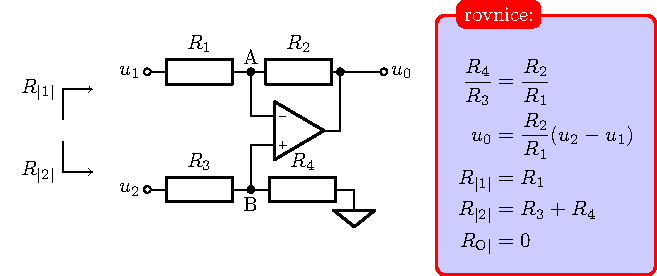
\includegraphics[width=\linewidth]{diff_opamp01.pdf}
          \caption{Rozdílový zesilovač. Podmínky potlačení souhlasné složky vstupních napětí $u_1$ a 
            $u_2$ je poměrové vyvážení zpětnovazebních rezistorů, $R_4/R_3 = R_2/R_1$. S ohledem na 
            ofset se obvykle volí uplná symetrie, tj. $R_4 = R_2$ a $R_3 = R_1$.}
          \label{AES:fig_diff_opamp01}
        \end{figure}

        Současné působení obou vstupních napětí ve vyváženém operačním obvodě
        $$\frac{R_4}{R_3}=\frac{R_2}{R_1},$$ přísluší výstupní napětí 
        \begin{equation}\label{AES:eq_diff_opamp}
          u_2 = \frac{R_2}{R_1}(u_2-u_1),   
        \end{equation}
        úměrné rozdílu vstupních napětí bez ohledu na jejich absolutní velikost. Odtud název 
        operačního obvodu. Důvod zařazení napěťového děliče ($R_3$,$R_4$) je zřejmý - dělič 
        sjednocuje zesílení invertujícího a neinvertujícího vstupu, která se liší absolutně o 
        jednotku. 
        
        Dvěma vstupům přísluší dva vstupní odpory. První vstupní odpor
        $$R_{\abs{1}} = R_1$$ je roven velikosti rezistoru $R_1$, protože vnitřní odpor bodu
        $A$\footnote{obdoba virtuální země} je nulový. Druhý vstupní odpor $$R_{\abs{2}} = R_3 +
        R_4$$ je roven součtu rezistorů $R_3$ a $R_4$, protože vnitřní odpor zbytku operačního
        obvodu v bodě $B$ je nekonečný. Tyto dva vstupní odpory jsou různé, i když jsou obě větve
        ($R_1$, $R_2$) a ($R_3$, $R_4$) stejné. 
        
        Vstupní odpory $R_{\abs{1}}$ a $R_{\abs{2}}$ přísluší dvěma samostatným uzemněným zdrojům 
        signálových napětí $u_1$ a $u_2$ podle \ref{AES:fig_diff_opamp01}. Volnému (izolovanému) 
        signálovému napěťovému zdroji připojenému diferenčně mezi vstupy rozdílového zesilovače, by 
        příslušel diferenční vstupní odpor $$R_{\abs{D}} = R_1 + R_3,$$ rovný součtové velikosti 
        rezistorů $R_{\abs{1}}$ a $R_{\abs{3}}$, protože body $A$ a $B$ jsou virtuálně zkratovány.

  \section{Analýza reálného operačního obvodu}\label{aesIchIVsecII}
  \section{Statické a dynamické chyby ve frekvenční oblasti}\label{aesIchIVsecIII}
  \section{Dynamické chyby v časové oblasti}\label{aesIchIVsecIV}
  \section{Vstupní a výstupní impedance}\label{aesIchIVsecV}
  \section{Ofset}\label{aesIchIVsecVI}
  \section{Šum}\label{aesIchIVsecVII}
  \section{Stabilita}\label{aesIchIVsecVIII}
%---------------------------------------------------------------------------------------------------
